\documentclass[10pt,twocolumn]{article}

% use the oxycomps style file
\usepackage{oxycomps}
\usepackage{amsmath}
\usepackage{graphicx}
\usepackage{url}

% usage: \fixme[comments describing issue]{text to be fixed}
% define \fixme as not doing anything special
\newcommand{\fixme}[2][]{#2}
% overwrite it so it shows up as red
\renewcommand{\fixme}[2][]{\textcolor{red}{#2}}
% overwrite it again so related text shows as footnotes
%\renewcommand{\fixme}[2][]{\textcolor{red}{#2\footnote{#1}}}

% read references.bib for the bibtex data
\bibliography{references}

% include metadata in the generated pdf file
\pdfinfo{
    /Title (Creating a Basic Biquad Filter Audio Plug-In with RNBO)
    /Author (August Ross)
}

% set the title and author information
\title{Creating a Basic Biquad Filter Audio Plug-In with RNBO}
\author{August Ross}
\affiliation{Occidental College}
\email{aross3@oxy.edu}

\begin{document}

\maketitle

\section{Introduction}

This tutorial paper presents a comprehensive guide on developing a Biquad filter audio plug-in within the RNBO \cite{RNBO} framework in MaxMSP (an audio programming environment), culminating in a fully operational VST3/AU plug-in compatible across major operating systems including PC, Mac, and Linux and the majority of commercial and open-source DAWs (Digital Audio Workstations). The primary objective is to empower readers with the skills to transform an initial concept into a commercial or personal audio software tool. This endeavor not only serves as a practical introduction to audio software development in MaxMSP but also aligns with broader academic goals, exploring a method of converting theoretical audio processing concepts into usable software products. By the tutorial's completion, a successful outcome is defined as the creation of a functioning plug-in.

This tutorial is also linked to my comprehensive project aims, which (while still being revised and fine-tuned) currently explores the process of transforming algorithms from audio processing research papers, or original algorithms, into practical software solutions, utilizing MaxMSP as the primary platform. By demonstrating the development of a Biquad filter audio plug-in — a fundamental component in audio signal processing (such as being at the core of equalizers, reverbs, and de-essers) — this tutorial embodies the initial steps toward achieving my broader comps objectives. It serves as a real example of how complex theoretical concepts can be converted into real-world applications, thus bridging the gap between academic research and practical utility in audio technology.

\section{Methods}

The initial step in creating this specific audio plug-in involves deciding on the specific filter design. For this project, a basic Biquad filter (a "two-pole, two-zero" filter. The term "biquad" itself comes from "bi-quadratic" which refers to the quadratic nature of both the filter's numerator and denominator when expressed as a transfer function \cite{Smith}) design was chosen due to its versatility and widespread application in digital audio processing (most notability in equalizers for shaping the frequency content of audio which is how it will be used in this plug-in). The Biquad filter is defined by the following difference equation:

\begin{align}
    y[n] &= a_0 \times x[n] + a_1 \times x[n-1] + a_2 \times x[n-2] \nonumber \\
         &\quad - b_1 \times y[n-1] - b_2 \times y[n-2]
\end{align}

Or by the following block diagram:

\begin{figure}[htbp]
  \centering
  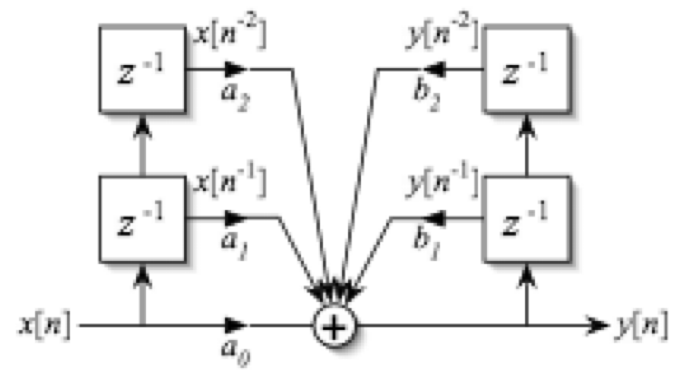
\includegraphics[width=0.8\linewidth]{biquad.png}
  \caption{A basic biquad filter as a block diagram. \cite{MaxMSPBiquad}}
  \label{fig:biquad}
\end{figure}

In this difference equation, input signals (x[n]) are transformed into output signals (y[n]) through specific coefficients ($a_0{_-}{_2}$ and $b_1{_-}{_2}$), laying the foundation for the filter's implementation in the RNBO work environment\cite{SmithDiff}.
\subsection{Initialization}
After determining the Biquad filter design, the next phase involves initializing the working environment. This was achieved by opening an empty RNBO patcher in MaxMSP, specifically tailored for audio effect plugin development rather than instrument based plugin development. This entails creating two audio inlets and two outlets to accommodate stereo processing, implemented as \verb|[in~ 1]|, \verb|[in~ 2]|, \verb|[out~ 1]|, and \verb|[out~ 2]| respectively. This setup forms the essential input-output structure for real-time audio signal processing, allowing the filter to modify audio passing through from left to right channels.
\subsection{User Interaction}
The design of user interactions with the plug-in plays a pivotal role in its functionality and user experience. Initially, controlling the filter through direct coefficient manipulation ($a_0$, $a_1$, etc.) was considered. However, this approach was deemed overly complex for end-users, who typically require intuitive control over the filter's characteristics rather than raw mathematical parameters.

Therefore, the decision was made to implement more user-friendly controls, which translate to common filter parameters: frequency, quality (Q factor), gain, and filter type (ex. low-pass, high-pass, band-pass). These were implemented using RNBO’s \verb|[param]| objects with specified ranges and default settings~\ref{tbl:parameters}, ensuring user safety and convenience by preventing the filter from reaching unstable states ("blowing up"). Notably, the frequency parameter was assigned an exponential scale (exponent: 3.3) to reflect the logarithmic nature of human hearing, improving usability by offering finer control over lower frequencies.

\begin{table}
    \footnotesize
    \begin{tabular}{|l|l|l|l|}
        \hline
        \textbf{Parameter}       &  \textbf{Min Value} & \textbf{Max Value}  &  \textbf{Initial Value}          \\
        \hline
        \textbf{Center Frequency (Hz)}  &  60.0 Hz         & 22.05 kHz &  6.0 kHz  \\
        \textbf{Quality/Q Factor}     &  0.01                & 10.0 &  1.0              \\
        \textbf{Gain}                  &  0.01         & 8.0 &  1.0     \\
        \textbf{Type}                  &  - &  -                &  Low-pass                \\
        \hline
    \end{tabular}
    \caption{The selected parameters and their respective min/max/default values. The default settings were selected to be a subtle low-pass filter at 6kHz.}
    \label{tbl:parameters}
\end{table}

\subsection{Algorithm Implementation in \texttt{[gen\textasciitilde]}}
Within the \verb|[rnbo~]| patcher, I initiated a new \verb|[gen~]| patcher environment to take advantage of the more advanced signal processing features it provides (such as single sample delays and sample rate based value updates). I first declared seven inlets; the initial two dedicated to audio input and the subsequent five designated for the filter coefficients. For output, two outlets were formulated for the stereo audio signals to traverse back to the parent \verb|[rnbo~]| patcher. The pivotal stage involved transcribing the biquad filter's block diagram~\ref{fig:biquad} into the \verb|[gen~]| environment. This translation required a rotation of the visual diagram by 90 degrees clockwise to align with the block programming paradigm of MaxMSP. In this framework, the \(z^{-1}\) elements, indicative of single sample delays, were adeptly represented using the \texttt{[history]} object. Furthermore, the diagram's triangular symbols, denoting amplitude adjustments, were interpreted as multiplication operations within the signal processing chain, typically ranging between -2.0 and 2.0 to modify the signal's amplitude effectively.

\begin{figure}[htbp]
  \centering
  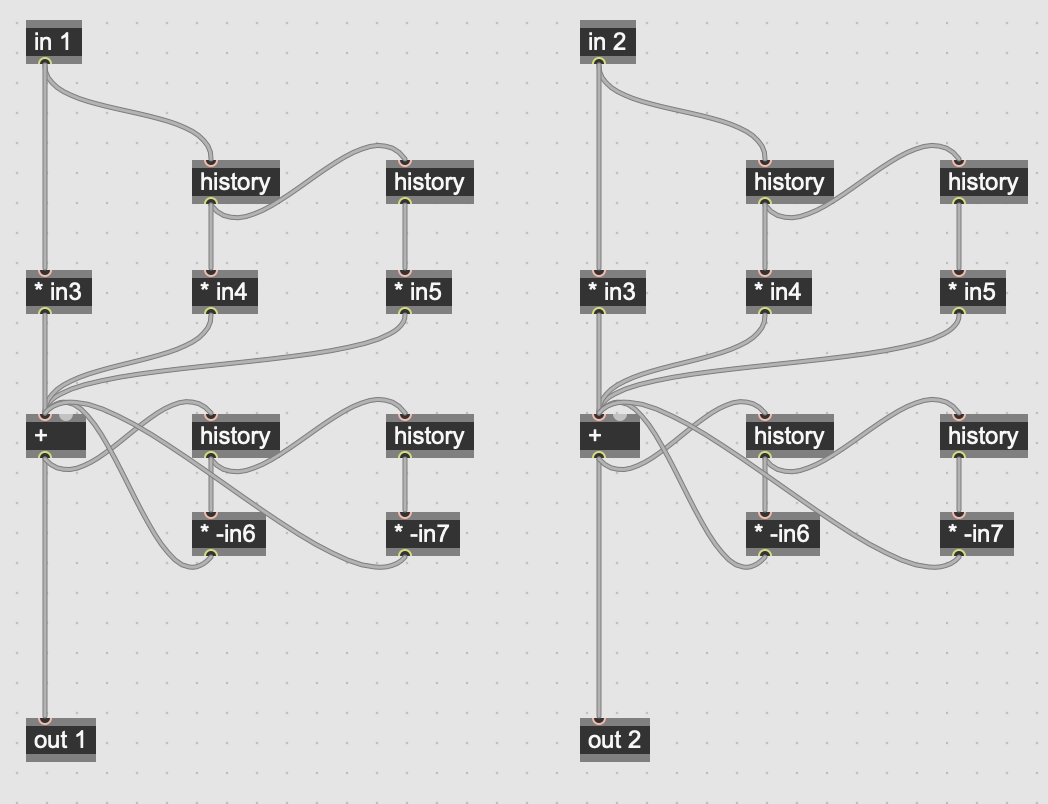
\includegraphics[width=0.8\linewidth]{biquadgen.png}
  \caption{The resulting biquad filter rebuilt in \texttt{[gen\textasciitilde]}.}
  \label{fig:biquadgen}
\end{figure}

\subsection{Parameter Conversion and Testing}
Transitioning from theoretical framework to practical application, I utilized the \texttt{[filtercoeff\textasciitilde]} object to translate user-defined parameters—center frequency, quality, and gain—into corresponding filter coefficients. This decision to employ a built-in object circumvented the intricate manual computation of these coefficients, aligning with the tutorial's scope. Post integration of the user parameters into the \texttt{[filtercoeff\textasciitilde]}, which was subsequently connected to the \verb|[gen~]| object, the setup was primed for auditory evaluation. I orchestrated a rudimentary audio playback system within the parent Max patcher, enabling the real-time auditory examination of the filter's response to varied parameter adjustments.

\begin{figure}[htbp]
  \centering
  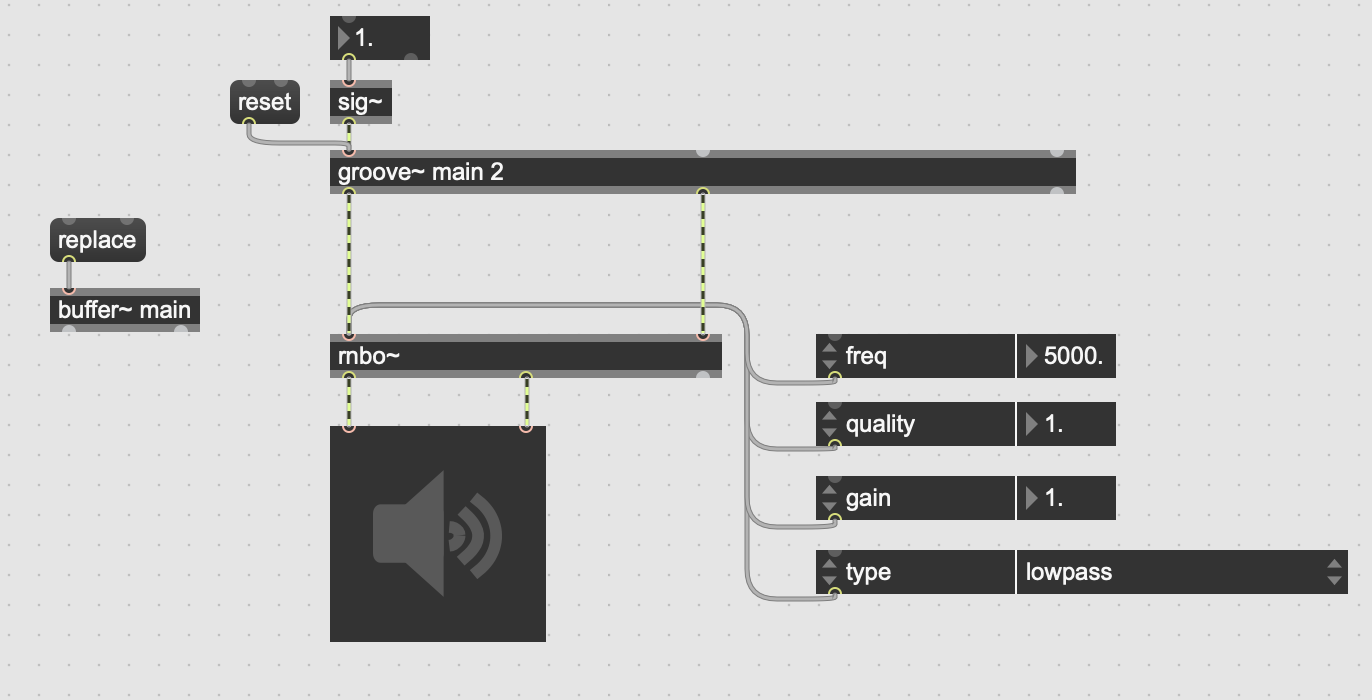
\includegraphics[width=0.8\linewidth]{audioplayback.png}
  \caption{The audio playback system used to test the algorithm. The \texttt{[groove\textasciitilde]} object plays back the file stored in the \texttt{[buffer\textasciitilde]} object.}
  \label{fig:playback}
\end{figure}

\subsection{Exporting to VST}
Satisfied with the auditory tests, I proceeded to encapsulate the project into a VST3 format, leveraging RNBO's export functionality. This phase offered two distinct pathways: direct export for C++ utilization within JUCE or a streamlined RNBO export that automates the conversion to VST format. I opted for the latter, since I didn't need any of the additional GUI enhancements or external library dependencies that JUCE provides, I specified the export settings tailored to my operating system (macOS) and initiated the VST3 compilation process. Upon completion, the newly created VST3 plugin was relocated to the designated system directory (Library/Audio/Plug-Ins/VST3/) for VST3s on macOS. The final validation ensued in my DAW (Ableton), where, post plugin re-scan, the custom biquad filter plug-in surfaced within the DAW environment, fully operational with all predefined settings intact, thereby affirming the successful culmination of the plugin development tutorial.

\begin{figure}[htbp]
  \centering
  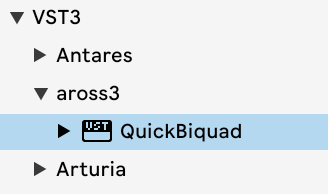
\includegraphics[width=0.8\linewidth]{vst.png}
  \caption{The VST3 showing up in my DAW with the given company and plug-in name being recognized correctly.}
  \label{fig:vstdaw}
\end{figure}

\begin{figure}[htbp]
  \centering
  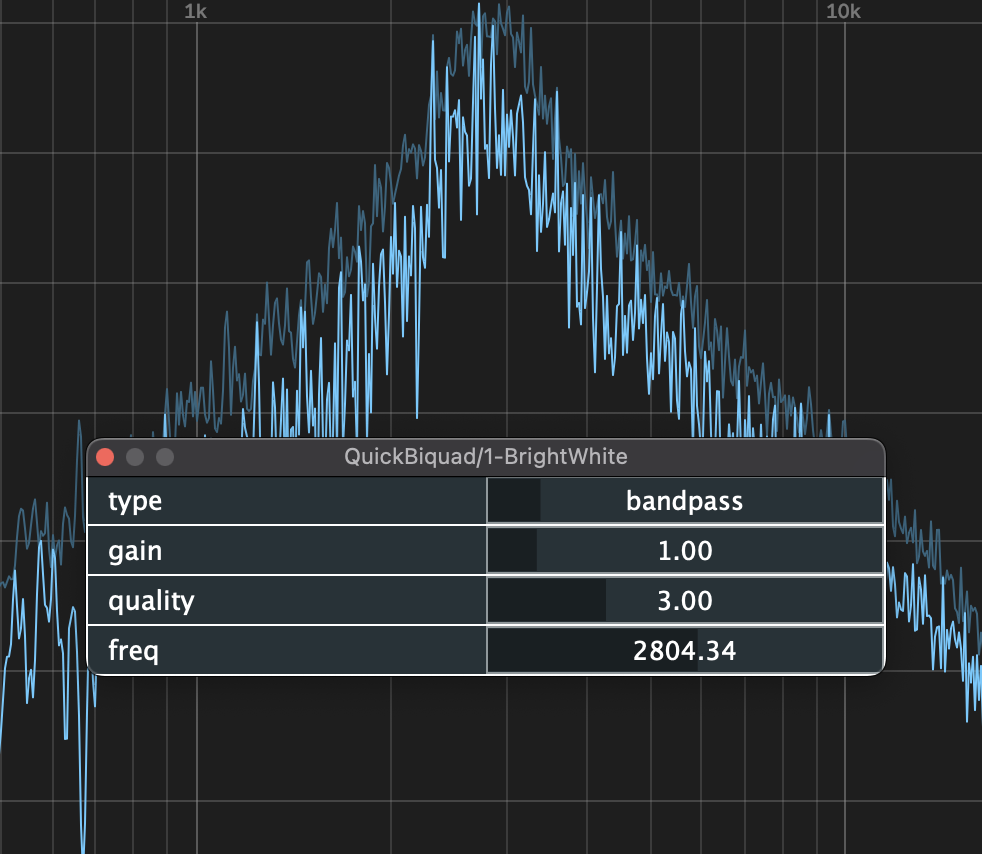
\includegraphics[width=0.8\linewidth]{bandpass2.png}
  \caption{Live spectrum results of white noise running through the bandpass setting on the plug-in in my DAW showing perfectly accurate results.}
  \label{fig:results}
\end{figure}

\section{Metrics and Results}

Success for this project was quantitatively measured by the functional completeness and performance accuracy of the developed VST plugin. The primary metric was the transition from a concept to a fully operational VST plugin, as proven by its integration and functionality within a Digital Audio Workstation (DAW). This achievement was visually verified through screenshots in the preceding sections, showcasing the plugin's operational status within the DAW environment.

\subsection{Performance Analysis}
To validate the filter's performance beyond mere functional integrity, an assessment was conducted within the Max environment. By subjecting a white noise signal to the filter, and subsequently analyzing the output's spectrum, I was able to compare the theoretical expectations against the empirical results. This analysis relied on matching the post-filter spectral characteristics with the predefined filter settings, a method that effectively illustrated the filter's response and its adherence to the expected behavior\cite{Jackson}.

\begin{figure}[htbp]
  \centering
  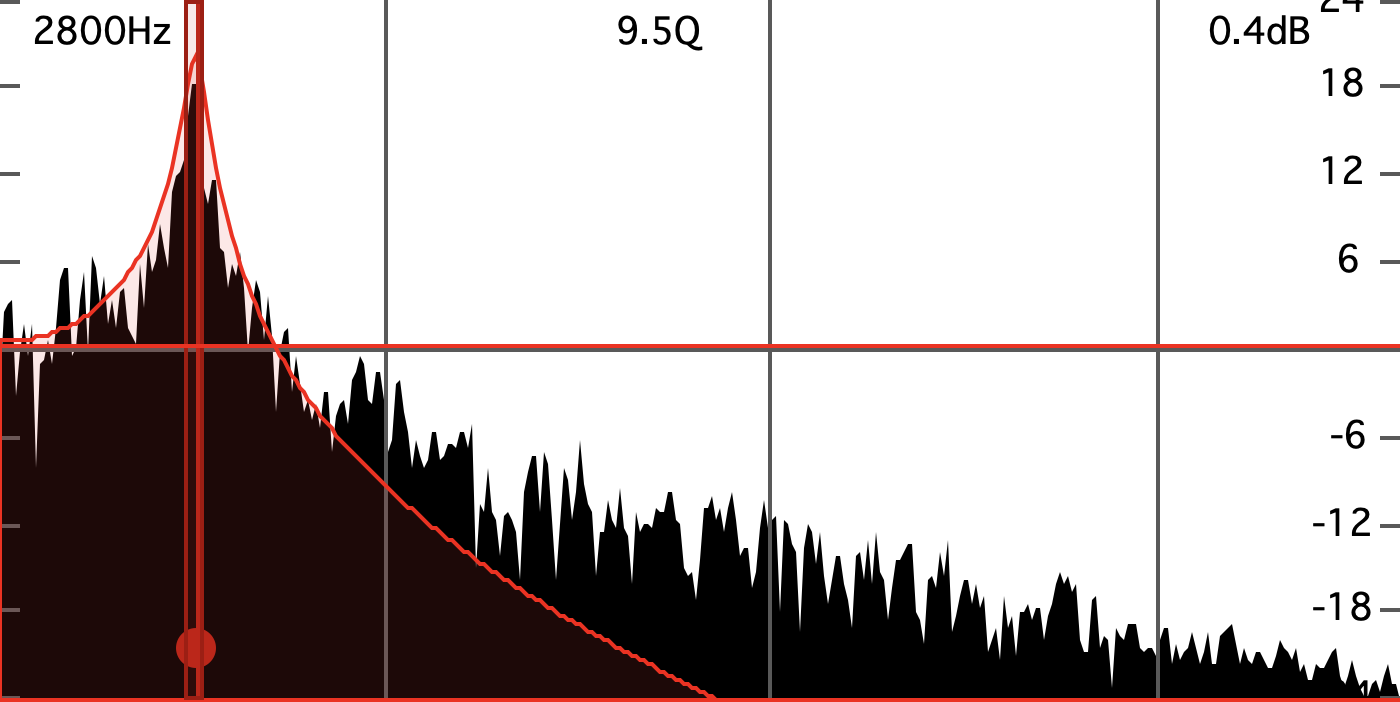
\includegraphics[width=0.8\linewidth]{spectrum.png}
  \caption{A further analysis in MaxMSP revealed that the biquad filter was fully accurate to input filter settings (in red). In black is the sculpted white noise output.}
  \label{fig:spectrummax}
\end{figure}

\begin{figure}[htbp]
  \centering
  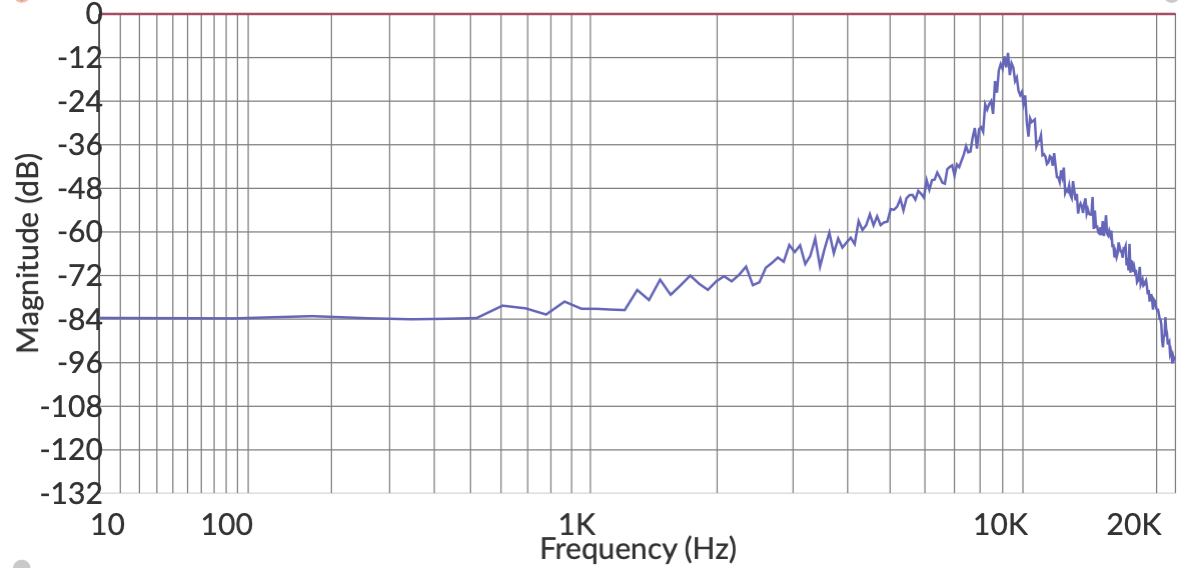
\includegraphics[width=0.8\linewidth]{fft2.png}
  \caption{Another FFT plotted analysis of white noise running through the bandpass filter setting with center frequency at 10kHz.}
  \label{fig:fft}
\end{figure}

\subsection{Interpretation of Results}
The fidelity of the output spectrum to the anticipated filter settings not only confirmed the plugin's operational success but also underscored the underlying RNBO framework in accurately translating digital signal processing concepts into practical audio tools.

This successful implementation illuminates broader implications for audio software development. By leveraging the RNBO environment's efficiency and the intuitive \verb|[gen~]| patching system, developers are provided with the capability to rapidly prototype and refine DSP algorithms. This paves the way for a more dynamic and innovative approach to plugin development, where ideas can transition from concept to usable software. Consequently, this tutorial not only validates the biquad filter's implementation as a pedagogical success but also as an example to the practical viability of MaxMSP and RNBO for crafting professional-grade audio solutions.

\section{Reflection}

Reflecting on the process of developing this audio effect plug-in, I am filled with a sense of accomplishment and enthusiasm towards my comprehensive project (comps) topic. Delving into the documentation and architectural quirks of biquad filters presented a solid challenge, primarily due to my initial unfamiliarity with their construction. However, the successful translation of theoretical knowledge into a functioning piece of software has been profoundly satisfying and enlightening.

As I pivot towards my comps, my feelings are predominantly positive, especially after the practical insights and skills garnered from this tutorial. Nonetheless, a lingering concern remains: the formalization and approval of my comps topic. The desire to begin tangible experimentation and development is strong, yet it is reliant upon establishing a clear and approved research direction.

In conclusion, the tutorial journey, while challenging, has been immensely rewarding, consolidating my interest in pursuing audio software development for my comps. My main endeavor moving forward is to solidify my comps topic.


\printbibliography

\end{document}
